\documentclass[10pt]{article}
\usepackage[T1]{fontenc}
\usepackage[utf8]{inputenc}
\usepackage{lmodern}
\usepackage[margin=0.7in]{geometry}
\usepackage{amsmath,amssymb}
\usepackage{microtype}
\usepackage{enumitem}
\usepackage{graphicx}
\usepackage{float}
\usepackage{booktabs,array}
\usepackage[font=small,labelfont=bf,skip=3pt]{caption}
\captionsetup[figure]{font=footnotesize}
\usepackage[dvipsnames]{xcolor}
\usepackage[backend=bibtex,style=authoryear,natbib=true,maxcitenames=2,maxbibnames=4,minbibnames=3,uniquelist=false,uniquename=false,giveninits=true,doi=false,isbn=false,url=false,eprint=false]{biblatex}
\addbibresource{refs.bib}
\usepackage[colorlinks=true,linkcolor=MidnightBlue,citecolor=MidnightBlue,urlcolor=MidnightBlue]{hyperref}
\usepackage[capitalise,nameinlink]{cleveref}
\setlength{\parskip}{2pt}
\setlength{\parindent}{0pt}
\setlist{nosep,leftmargin=*}
\setlength{\textfloatsep}{8pt}
\setlength{\intextsep}{6pt}
\makeatletter
\renewcommand\paragraph{\@startsection{paragraph}{4}{\z@}{1.0ex \@plus .3ex \@minus .2ex}{-1em}{\normalfont\normalsize\bfseries}}
\renewcommand\maketitle{\begin{center}{\large\bfseries\@title\par}\vspace{3pt}\@author\quad\textperiodcentered\quad\@date\end{center}}
\makeatother

\title{How AdamW and Muon Train a Small Language Model\\[1pt]
\normalfont Initial checkpoint with the MSE loss, MIT 6.7910, Fall 2026}
\author{Juntang Wang and V\'ictor Conchello}
\date{November 14, 2026}

\begin{document}
\maketitle
\vspace{-0.8em}

\paragraph{Summary.} We train a small language model with AdamW and Muon from one initialization, on the same
mini-batches, with the mean squared error (MSE) loss. (1)~Muon trains faster. Its path and final model differ from
AdamW's about as much as two runs of one optimizer on different mini-batches, but its loss is lower. (2)~The optimizers
differ in various metrics that look at the model's internals: weight spectra, similarity of consecutive updates,
curvature, and MLP sparsity. (3)~When a run switches optimizer mid-training, the similarity of its consecutive updates
ends at the new optimizer's level. Its weight spectra, MLP sparsity and curvature depend on when it switches: a switch
to Muon after 400 AdamW steps keeps AdamW's low stable rank, while one to AdamW within 1500 steps leaves little trace.

\paragraph{Setup.} \emph{Model.} We train a 14M-parameter nanoGPT \citep{karpathy2022nanogpt} on TinyStories
\citep{eldan2023tinystories} for 10{,}000 steps of 128 sequences of 256 tokens (settings: \cref{app:hparams}).
\emph{Loss.} Instead of cross-entropy, every run minimizes the MSE $\|z-e_y\|^2$ between the 4096 outputs $z$ and the
one-hot next token $e_y$. The model predicts $p=\max(z,0)/\sum_v\max(z_v,0)$.

\emph{Optimizers.} Muon \citep{jordan2024muon} orthogonalizes the update of each weight matrix in the transformer
blocks: it sets its singular values to about 1. In Muon runs, AdamW trains the other parameters. Each optimizer runs
from the same weights on the same five \emph{data orders} (mini-batch sequences), at its best learning rate with no
stuck run (\cref{tab:app-optim}).

\paragraph{Step 1: how the trajectories differ (\cref{fig:div}).} \emph{Comparing runs.} The distance between two runs
is the mean Jensen--Shannon divergence (JS, in bits) of their next-token predictions on held-out text. We compare runs
at equal step and at equal training loss; at equal loss, speed does not count as a difference. The \emph{floor} is the
mean distance between two data orders of one optimizer. A distance of one floor means ``as different as two data
orders''.

\begin{figure}[H]
\centering
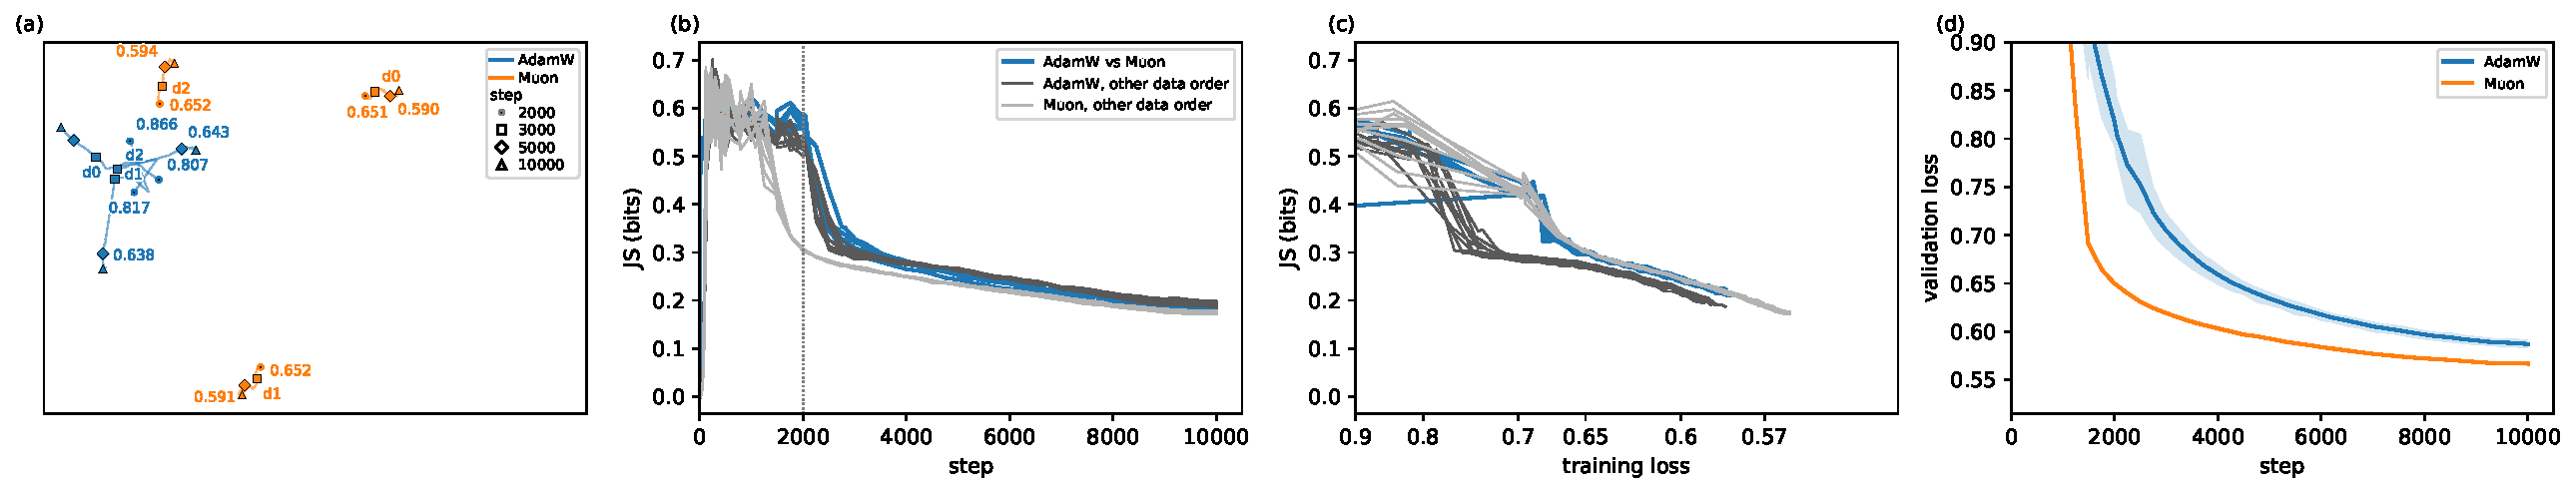
\includegraphics[width=\linewidth]{figures_mse/divergence_umap_adamw_muon.pdf}
\caption{AdamW and Muon. (a) Checkpoints from step 2000 on, mapped to 2-D by densMAP (shows neighbours, not distances);
labels: training loss and data order. (b) JS between runs at equal step. (c) The same at equal training loss. (d)
Validation loss.}
\label{fig:div}
\end{figure}

\emph{Faster, and on a different path.} Muon reaches AdamW's final validation loss (0.587 on average) by step 5750 (d).
Since they share the initialization and batches, if Muon just followed AdamW's path faster, they would be closer at
equal loss (c) than at equal step (b). The opposite happens: from step 3000 on, their distance is larger at equal loss
than at equal step (at AdamW's step 5000, 0.285 against 0.252). So the paths differ. Their distance is about that of two
data orders: at equal step, AdamW and Muon on one data order are closer than two data orders of AdamW and farther apart
than two of Muon (step 5000: 0.252 against 0.264 and 0.233; b).

\emph{Endpoints.} The final models are about one floor apart (b), but Muon's validation loss is lower: 0.567 against
0.587 (d).

\paragraph{Step 2: what differs along the way.} We measure 30 properties of each model at 34 points of training, in five
groups: weights $W$, one-step updates $\Delta W$, loss curvature (Hessian $H$), internal activations and predictions
(\cref{app:metrics} defines each metric and compares all of them in \cref{tab:app-am,tab:app-sgd}). \Cref{tab:app-sgd}
also gives the values for SGD with momentum.

We compare the optimizers by each metric's ratio AdamW/Muon at training loss 0.65, on three data orders each
(\cref{fig:rank}, \cref{tab:app-am}). The $\pm$ gives its range over data orders; if it excludes 1, the optimizers
differ more than data orders do.

\begin{figure}[H]
\centering
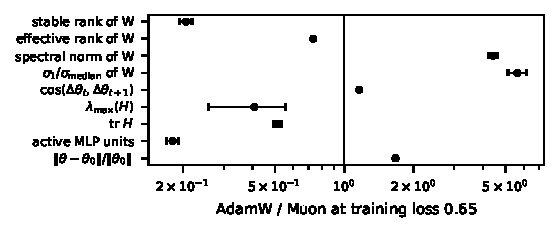
\includegraphics{figures_mse/ranking.pdf}
\caption{Ratio AdamW/Muon at training loss 0.65, for selected metrics; three data orders each; bars: range across data
orders.}
\label{fig:rank}
\end{figure}

\begin{itemize}
\item \emph{Weights $W$.} Muon's weight matrices have more evenly sized singular values. Their stable rank
$\|W\|_F^2/\|W\|_2^2$ is 85 against AdamW's 17 (Muon/AdamW $4.9\pm0.3$), and their effective rank 320 against 234. Their
spectral norm (2.0 against 9.1) and largest-to-median singular-value ratio $\sigma_1/\sigma_{\rm median}$ (2.9 against
16.5) are lower. AdamW also moves farther from the initialization: 2.7 against 1.6 times the initial norm.
\item \emph{One-step updates $\Delta W$.} Consecutive Muon steps are less alike (cosine 0.76 against 0.88). Their stable
rank is much higher (208 against 11; \cref{tab:app-am}), but by construction: Muon orthogonalizes every update.
\item \emph{Loss curvature (Hessian $H$).} Muon is sharper: the top Hessian eigenvalue $\lambda_{\max}$ is 107 against
40, the trace $\operatorname{tr}H$ 4380 against 2260. Muon's steps are also larger relative to the weights
($\|\Delta\theta\|/\|\theta\|$ is $4.8\cdot10^{-3}$ against AdamW's $3.5\cdot10^{-3}$).
\item \emph{Internal activations.} AdamW's MLP is much sparser: 8\% of its units are active, against 43\% for Muon.
\item \emph{Predictions.} AdamW's are more concentrated (entropy 4.59 nats against 4.95). The loss on frequent targets
does not separate the two (\cref{tab:app-am}).
\end{itemize}

\paragraph{Step 3: swaps (\cref{fig:swap}).} \emph{Swaps.} A \emph{swap} switches a run of one optimizer (the
\emph{parent}, on data order 0) to the other optimizer at a \emph{fork step}, then trains it to step 10{,}000 on the
parent's batches (\cref{app:forks} gives the fork steps, the optimizer state at the swap and the measurement steps). An
optimizer's \emph{own run} is its run from the start. We swap at nine fork steps from 50 to 4000, in both directions. We
give each metric's value at step 10{,}000 as a fraction of the way, on a linear scale, from the parent's value (0) to
that of the new optimizer's own run (1).

\begin{figure}[H]
\centering
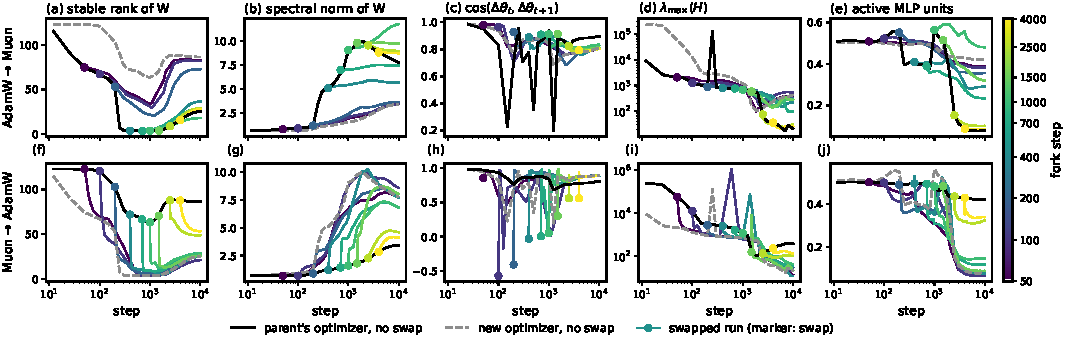
\includegraphics[width=\linewidth]{figures_mse/swap_traj_adamw_muon.pdf}
\caption{Swaps on data order 0: five metrics against the step. Top: AdamW to Muon; bottom: Muon to AdamW. Black: the
parent's optimizer without a swap; grey dashed: the new optimizer's own run; colour: swapped runs, by fork step (dot:
the swap).}
\label{fig:swap}
\end{figure}

\emph{Weights $W$ and internal activations.} For the spectral norm and stable rank of $W$ (a, b, f, g) and the fraction
of active MLP units (e, j), the final value depends on the fork step. AdamW's own stable rank falls from 53 to 4 between
steps 200 and 300 (a). Swaps to Muon before this fall end near Muon's own run (0.78--0.94 of the way); later ones stay
near AdamW's (at most 0.19). Swaps to AdamW at fork steps up to 1500 end at AdamW's stable rank (0.94--1.07), and those
at steps 2500 and 4000 about half-way. So a few hundred AdamW steps largely fix the final stable rank, while 1500 Muon
steps do not.

\emph{One-step updates $\Delta W$.} The cosine between consecutive updates ends at the new optimizer's level in all 18
swaps (c, h): 0.80--0.83 after a switch to Muon and 0.89--0.90 after a switch to AdamW (own runs: 0.81 and 0.89). This
is expected: it reflects the optimizer's own dynamics more than the model's weights.

\emph{Loss curvature (Hessian $H$).} $\lambda_{\max}$ also depends on the fork step (d, i). Swaps to AdamW up to step
1500 fall to AdamW's level (0.94--1.02 of the way); those at steps 2500 and 4000 end 0.78 and 0.70 of the way. Swaps to
Muon end near or above Muon's level up to step 200 (0.81--1.38), part of the way at steps 400 to 1500 (0.21--0.69), and
at AdamW's level at steps 2500 and 4000 (0.03 and 0.01).

\paragraph{Next steps.} (i)~Repeat Steps 1--3 on a larger model (TinyStories-30M) and on character-level Shakespeare.
(ii)~For each property that differs in Step 2: does it follow directly from Muon's orthogonalized updates, or does it
emerge during training? (iii)~Do these differences explain Step 1, Muon's faster training and different path? Is any of
them a reason Muon does better?

\clearpage
\printbibliography

\clearpage \appendix
%% Appendix of checkpoint_mse.tex, \input right after \appendix.
\crefalias{section}{appendix}\crefalias{subsection}{appendix}
\section{Hyperparameters}
\label{app:hparams}

\begin{center}\small
\captionsetup{type=table}
\caption{Hyperparameters shared by the AdamW and Muon runs.}
\label{tab:app-shared}
\begin{tabular}{@{}lp{0.74\linewidth}@{}}
\hline
Runs & AdamW and Muon $\times$ data orders d0--d4 (10) \\
\hline
Model & nanoGPT, pre-LayerNorm blocks \\
Layers, heads, width & 6, 6, 384 \\
MLP & GELU, width 1536 \\
Biases, dropout & none, none \\
Output head & untied \\
Attention projections & separate query, key, value \\
Context & 256 tokens \\
Parameters & 13.9M (10.6M without token and position embeddings and head) \\
\hline
Data & TinyStories (GPT-4 version) \\
Tokenizer & byte-level BPE, 4096 tokens, trained on the training split \\
Batch & 128 windows $\times$ 256 tokens \\
Window offsets & from the training split; generator seeded with (data order, step), same for every optimizer \\
\hline
Loss & MSE: $\|z-e_y\|^2$, summed over the 4096 outputs $z$ (no softmax) and averaged over positions; $e_y$ is the
  one-hot vector of the next token \\
Steps & 10{,}000 \\
Tokens & 328M (about 0.6 epochs) \\
Learning rate & $\eta\,\varphi(t)$ at step $t$, every parameter group \\
Warmup & linear, $\varphi(t)=(t+1)/200$ for $t<200$ \\
Decay & cosine to $\varphi=0.1$ at step 10{,}000 \\
Gradient clipping & none \\
\hline
Initialization seed & 0, all runs \\
Training precision & bfloat16 autocast \\
Prediction, Hessian precision & float32, no autocast (TF32 matrix products allowed) \\
\hline
Logged predictions & next-token distributions $p=\max(z,0)/\sum_v\max(z_v,0)$ (uniform if no output is positive):
  128 fixed validation sequences $\times$ 16 evenly spaced positions (2{,}048), stored as float16 outputs $z$ \\
Training loss & 64 fixed training sequences, all positions; used to match runs at equal loss \\
Floor & mean JS between two data orders of one optimizer, at equal training loss; for two optimizers, the larger
  of their floors \\
Both logged at & every 250th step $+$ 30 log-spaced steps in $[1, 10{,}000]$ \\
\hline
Hessian & top eigenvalue, 20 Lanczos iterations, 32 fixed training sequences; AdamW also of
  $P^{-1/2}HP^{-1/2}$, with $P$ AdamW's diagonal preconditioner \\
Measured at & every 500th step $+$ 30 log-spaced steps \\
\hline
\end{tabular}
\end{center}

\begin{center}\small
\captionsetup{type=table}
\caption{Optimizer-specific hyperparameters. $n_{\rm out}$, $n_{\rm in}$: output and input size of the matrix.}
\label{tab:app-optim}
\setlength{\tabcolsep}{4pt}
\begin{tabular}{@{}p{0.2\linewidth}p{0.36\linewidth}p{0.4\linewidth}@{}}
\hline
 & AdamW & Muon \tabularnewline
\hline
$\eta$ & $2\cdot10^{-3}$ & $5\cdot10^{-3}$ \tabularnewline
$\eta$ choice & \raggedright second-best final validation loss of a 5-rate sweep on d0 (0.591); the best rate,
  $4\cdot10^{-3}$ (0.584), stays at 0.86 on d1 & \raggedright best final validation loss of a 7-rate sweep on d0
  \tabularnewline
Update & bias-corrected moments & \raggedright Nesterov momentum; 5 quintic Newton--Schulz steps in bfloat16 \tabularnewline
Momentum & $\beta=(0.9,0.95)$ & $\beta=0.95$ \tabularnewline
$\epsilon$ & $10^{-8}$ & -- \tabularnewline
Update scale & -- & $\sqrt{\max(1,n_{\rm out}/n_{\rm in})}$ \tabularnewline
Weight decay & \raggedright 0.1, decoupled; none on LayerNorm gains & none \tabularnewline
Parameters & all & \raggedright query, key, value, attention-output and both MLP matrices of every block \tabularnewline
\hline
Aux.\ AdamW & -- & embeddings, head, LayerNorm gains \tabularnewline
Aux.\ $\eta$, $\beta$, $\epsilon$ & -- & $2\cdot10^{-3}$, $(0.9,0.95)$, $10^{-8}$ \tabularnewline
Aux.\ weight decay & -- & none \tabularnewline
\hline
\end{tabular}
\end{center}

\section{Metrics}
\label{app:metrics}

The Step-2 runs save checkpoints every 1000 steps, at 12 log-spaced steps, and at three consecutive steps $t,t+1,t+2$
for 24 values of $t$ from 25 to 9998 (to measure one-step updates); we measure the metrics at 34 of these per run, and
the Step-3 swaps at the steps in \cref{tab:app-forks}. \emph{Weights}: for all parameters together, $\|\theta\|_2$,
$\|\theta-\theta_0\|/\|\theta_0\|$ and $\|\theta\|_\infty/\|\theta\|_2$; and, averaged over the 36 weight matrices
$W$ of the blocks, the stable rank $\|W\|_F^2/\|W\|_2^2$, the effective rank $\exp H(\sigma/\textstyle\sum\sigma)$
with $H$ the entropy of the normalized singular values $\sigma$, the spectral norm, and $\sigma_1/\sigma_{\rm median}$.
\emph{Updates} $\Delta\theta_t=\theta_{t+1}-\theta_t$: $\|\Delta\theta_t\|/\|\theta_t\|$, its cosine with
$\Delta\theta_{t+1}$ and with the negative gradient $-g_t$ on step $t$'s batch, and the stable and effective rank of
its block matrices $\Delta W$. \emph{Curvature} of the training loss on 32 fixed training sequences, with Hessian $H$:
$\lambda_{\max}(H)$ (20 Lanczos iterations, logged during training), $\operatorname{tr}H$ (10 Rademacher probes),
$\operatorname{tr}H/\lambda_{\max}$, and the batch sharpness $\mathbb{E}_B[g_B^\top H_Bg_B]/\mathbb{E}_B\|g_B\|^2$,
where $g_B$ and $H_B$ are the gradient and Hessian on a mini-batch $B$.
\emph{Predictions}, on the 2{,}048 held-out
positions: entropy, mean top-1 probability, calibration error (15 bins), top-1 accuracy, loss on the targets in the top
and the bottom third of training-set frequency and their difference, and JS to the unigram and to the bigram model
of the training split. \emph{Activations}, on 32 held-out sequences: attention entropy
and attention on the first token (means over layers, heads and positions), fraction of MLP pre-activations above 0,
RMS of the residual stream after the last block, and effective rank of the centred final features.

SGD, the reference in \cref{tab:app-sgd}, uses heavy-ball momentum 0.9 and learning rate 0.02, the best final
validation loss of ten rates from 0.001 to 0.3 on d0 (0.045 ends with all outputs at 0; 0.06 and above diverge);
everything else is as in \cref{tab:app-shared}. SGD learns little: its training loss ends at 0.96 on all three data
orders, and predicting every token by its frequency gives 0.986. So \cref{tab:app-sgd} compares the three optimizers
at training loss 0.97. AdamW and Muon pass this loss before step 1500, long before the loss 0.65 of
\cref{tab:app-am}.

\begin{center}\small\begin{minipage}{\linewidth}\centering
\captionsetup{type=table}
\caption{All metrics of Step 2 at training loss 0.65, which AdamW reaches near step 4600 and Muon near step 2000:
mean $\pm$ half-range over data orders 0--2, and the ratio AdamW/Muon. If AdamW's values range over $[a_{\min},a_{\max}]$ and Muon's over $[b_{\min},b_{\max}]$, the ratio
ranges over $[a_{\min}/b_{\max},\,a_{\max}/b_{\min}]$, given as midpoint $\pm$ half-width. Rows marked ($\times10^k$)
are in units of $10^k$. Bold: the five ratios farthest from 1 whose range excludes 1.}
\label{tab:app-am}
\footnotesize\setlength{\tabcolsep}{2.5pt}\setlength{\aboverulesep}{0pt}\setlength{\belowrulesep}{0pt}%
\renewcommand{\arraystretch}{1.15}%
\begin{tabular}{@{}l|cc|c@{}}
 & AdamW & Muon & A/M \\
\midrule
\emph{Weights $W$} & & & \\
weight norm $\|\theta\|_2$ & $260 \pm 4$ & $172 \pm 0$ & $1.51 \pm 0.03$ \\
distance from init.\ $/\|\theta_0\|$ & $2.68 \pm 0.05$ & $1.61 \pm 0.01$ & $1.67 \pm 0.04$ \\
largest entry $/\|\theta\|_2$ ($\times10^{-3}$) & $7.56 \pm 0.33$ & $8.02 \pm 0.05$ & $0.935 \pm 0.046$ \\
stable rank of $W$ & $17.2 \pm 1.0$ & $85.5 \pm 0.6$ & {\boldmath\textbf{$0.206 \pm 0.013$}} \\
effective rank of $W$ & $234 \pm 4$ & $320 \pm 0$ & $0.734 \pm 0.012$ \\
spectral norm of $W$ & $9.11 \pm 0.40$ & $2.04 \pm 0.00$ & $4.42 \pm 0.20$ \\
$\sigma_1/\sigma_{\rm median}$ of $W$ & $16.5 \pm 1.3$ & $2.87 \pm 0.02$ & {\boldmath\textbf{$5.64 \pm 0.51$}} \\
\emph{One-step updates $\Delta W$} & & & \\
step size $\|\Delta\theta\|/\|\theta\|$ ($\times10^{-3}$) & $3.51 \pm 0.13$ & $4.81 \pm 0.01$ & $0.727 \pm 0.028$ \\
stable rank of $\Delta W$ & $11.4 \pm 1.0$ & $208 \pm 1$ & {\boldmath\textbf{$(5.45 \pm 0.49){\times}10^{-2}$}} \\
effective rank of $\Delta W$ & $195 \pm 5$ & $361 \pm 1$ & $0.542 \pm 0.015$ \\
cosine of consecutive steps & $0.881 \pm 0.002$ & $0.760 \pm 0.000$ & $1.16 \pm 0.00$ \\
cosine of step and $-g$ & $0.185 \pm 0.005$ & $0.156 \pm 0.003$ & $1.20 \pm 0.06$ \\
\emph{Loss curvature (Hessian $H$)} & & & \\
top Hessian eigenvalue & $40.4 \pm 11.6$ & $107 \pm 10$ & $0.407 \pm 0.148$ \\
batch sharpness & $2.20 \pm 0.25$ & $10.1 \pm 3.0$ & $0.272 \pm 0.113$ \\
Hessian trace & $2260 \pm 50$ & $4380 \pm 90$ & $0.514 \pm 0.021$ \\
trace / top eigenvalue & $58.2 \pm 16.5$ & $41.1 \pm 4.0$ & $1.42 \pm 0.53$ \\
\emph{Internal activations} & & & \\
attention entropy (nats) & $2.36 \pm 0.30$ & $3.75 \pm 0.00$ & $0.628 \pm 0.080$ \\
attention on first token ($\times10^{-2}$) & $1.38 \pm 0.07$ & $1.52 \pm 0.01$ & $0.917 \pm 0.052$ \\
active MLP units ($\times10^{-1}$) & $0.792 \pm 0.043$ & $4.34 \pm 0.01$ & {\boldmath\textbf{$0.180 \pm 0.011$}} \\
residual-stream RMS & $40.1 \pm 3.6$ & $1.36 \pm 0.00$ & {\boldmath\textbf{$29.7 \pm 2.7$}} \\
effective rank of features & $231 \pm 2$ & $243 \pm 1$ & $0.951 \pm 0.012$ \\
\emph{Predictions} & & & \\
prediction entropy (nats) & $4.59 \pm 0.01$ & $4.95 \pm 0.01$ & $0.926 \pm 0.004$ \\
mean top-1 probability & $0.306 \pm 0.002$ & $0.282 \pm 0.001$ & $1.09 \pm 0.01$ \\
calibration error & $0.165 \pm 0.004$ & $0.180 \pm 0.004$ & $0.919 \pm 0.045$ \\
top-1 accuracy & $0.470 \pm 0.004$ & $0.461 \pm 0.003$ & $1.02 \pm 0.02$ \\
loss on frequent targets & $0.378 \pm 0.007$ & $0.379 \pm 0.005$ & $1.00 \pm 0.03$ \\
loss on rare targets & $0.987 \pm 0.004$ & $0.997 \pm 0.002$ & $0.989 \pm 0.006$ \\
rare minus frequent loss & $0.609 \pm 0.011$ & $0.619 \pm 0.007$ & $0.979 \pm 0.028$ \\
JS to unigram model & $0.564 \pm 0.003$ & $0.568 \pm 0.002$ & $0.995 \pm 0.007$ \\
JS to bigram model & $0.466 \pm 0.003$ & $0.487 \pm 0.001$ & $0.954 \pm 0.008$ \\
\end{tabular}\end{minipage}
\end{center}

\begin{center}\small\begin{minipage}{\linewidth}\centering
\captionsetup{type=table}
\caption{The metrics of \cref{tab:app-am} at training loss 0.97, with SGD as a reference: ratios AdamW/SGD and
Muon/SGD. Bold: in each ratio column, the five ratios farthest from 1 whose range excludes 1.}
\label{tab:app-sgd}
\footnotesize\setlength{\tabcolsep}{2.5pt}\setlength{\aboverulesep}{0pt}\setlength{\belowrulesep}{0pt}%
\renewcommand{\arraystretch}{1.15}%
\begin{tabular}{@{}l|ccc|cc@{}}
 & AdamW & Muon & SGD & A/S & M/S \\
\midrule
\emph{Weights $W$} & & & & & \\
weight norm $\|\theta\|_2$ & $155 \pm 10$ & $126 \pm 0$ & $99.9 \pm 0.1$ & $1.53 \pm 0.10$ & $1.26 \pm 0.00$ \\
distance from init.\ $/\|\theta_0\|$ & $1.38 \pm 0.13$ & $0.977 \pm 0.001$ & $0.405 \pm 0.002$ & $3.33 \pm 0.34$ & $2.41 \pm 0.01$ \\
largest entry $/\|\theta\|_2$ ($\times10^{-2}$) & $0.837 \pm 0.050$ & $1.08 \pm 0.01$ & $1.02 \pm 0.00$ & $0.834 \pm 0.049$ & $1.06 \pm 0.01$ \\
stable rank of $W$ & $4.01 \pm 0.14$ & $64.1 \pm 0.3$ & $41.5 \pm 0.1$ & {\boldmath\textbf{$(9.61 \pm 0.35){\times}10^{-2}$}} & $1.55 \pm 0.01$ \\
effective rank of $W$ & $208 \pm 13$ & $315 \pm 0$ & $283 \pm 0$ & $0.741 \pm 0.048$ & $1.11 \pm 0.00$ \\
spectral norm of $W$ & $9.54 \pm 1.24$ & $1.62 \pm 0.00$ & $3.90 \pm 0.01$ & $2.42 \pm 0.33$ & $0.415 \pm 0.002$ \\
$\sigma_1/\sigma_{\rm median}$ of $W$ & $39.2 \pm 4.7$ & $3.58 \pm 0.01$ & $23.5 \pm 0.1$ & $1.64 \pm 0.21$ & $0.152 \pm 0.001$ \\
\emph{One-step updates $\Delta W$} & & & & & \\
step size $\|\Delta\theta\|/\|\theta\|$ ($\times10^{-3}$) & $5.87 \pm 0.13$ & $6.11 \pm 0.07$ & $0.0183 \pm 0.0050$ & {\boldmath\textbf{$322 \pm 90$}} & {\boldmath\textbf{$335 \pm 90$}} \\
stable rank of $\Delta W$ & $2.49 \pm 0.30$ & $63.5 \pm 1.0$ & $1.08 \pm 0.03$ & $2.37 \pm 0.33$ & {\boldmath\textbf{$58.3 \pm 2.4$}} \\
effective rank of $\Delta W$ & $56.9 \pm 6.2$ & $227 \pm 2$ & $35.5 \pm 1.1$ & $1.66 \pm 0.22$ & $6.44 \pm 0.24$ \\
cosine of consecutive steps & $0.798 \pm 0.093$ & $0.793 \pm 0.010$ & $0.699 \pm 0.168$ & $1.27 \pm 0.45$ & $1.25 \pm 0.32$ \\
cosine of step and $-g$ ($\times10^{-2}$) & $2.36 \pm 0.36$ & $4.99 \pm 0.10$ & $60.0 \pm 22.7$ & {\boldmath\textbf{$(4.73 \pm 2.31){\times}10^{-2}$}} & $(9.42 \pm 3.61){\times}10^{-2}$ \\
\emph{Loss curvature (Hessian $H$)} & & & & & \\
top Hessian eigenvalue & $635 \pm 11$ & $1200 \pm 10$ & $139 \pm 32$ & $4.69 \pm 1.13$ & $8.81 \pm 2.03$ \\
batch sharpness & $477 \pm 31$ & $869 \pm 9$ & $93.9 \pm 21.9$ & $5.31 \pm 1.55$ & $9.67 \pm 2.33$ \\
Hessian trace & $(1.83 \pm 0.14){\times}10^{6}$ & $(2.45 \pm 0.01){\times}10^{6}$ & $(1.62 \pm 0.05){\times}10^{4}$ & {\boldmath\textbf{$113 \pm 12$}} & {\boldmath\textbf{$152 \pm 5$}} \\
trace / top eigenvalue & $3080 \pm 130$ & $2110 \pm 60$ & $120 \pm 23$ & {\boldmath\textbf{$27.2 \pm 6.5$}} & {\boldmath\textbf{$18.7 \pm 4.2$}} \\
\emph{Internal activations} & & & & & \\
attention entropy (nats) & $1.73 \pm 1.09$ & $4.12 \pm 0.01$ & $4.58 \pm 0.00$ & $0.381 \pm 0.238$ & $0.900 \pm 0.001$ \\
attention on first token ($\times10^{-2}$) & $2.29 \pm 1.11$ & $1.85 \pm 0.01$ & $2.02 \pm 0.00$ & $1.30 \pm 0.55$ & $0.913 \pm 0.005$ \\
active MLP units & $0.430 \pm 0.082$ & $0.477 \pm 0.000$ & $0.465 \pm 0.001$ & $0.932 \pm 0.179$ & $1.03 \pm 0.00$ \\
residual-stream RMS & $274 \pm 89$ & $2.14 \pm 0.01$ & $66.0 \pm 1.5$ & $4.03 \pm 1.45$ & {\boldmath\textbf{$(3.26 \pm 0.09){\times}10^{-2}$}} \\
effective rank of features & $33.5 \pm 2.4$ & $105 \pm 1$ & $41.8 \pm 2.1$ & $0.810 \pm 0.100$ & $2.55 \pm 0.17$ \\
\emph{Predictions} & & & & & \\
prediction entropy (nats) & $7.25 \pm 0.02$ & $7.24 \pm 0.00$ & $6.51 \pm 0.02$ & $1.11 \pm 0.01$ & $1.11 \pm 0.00$ \\
mean top-1 probability ($\times10^{-2}$) & $2.69 \pm 0.10$ & $2.81 \pm 0.03$ & $5.68 \pm 0.14$ & $0.476 \pm 0.028$ & $0.494 \pm 0.017$ \\
calibration error ($\times10^{-1}$) & $1.47 \pm 0.07$ & $3.61 \pm 0.03$ & $0.436 \pm 0.020$ & $3.34 \pm 0.30$ & $8.30 \pm 0.43$ \\
top-1 accuracy & $0.174 \pm 0.007$ & $0.389 \pm 0.003$ & $0.100 \pm 0.001$ & $1.71 \pm 0.08$ & $3.88 \pm 0.05$ \\
loss on frequent targets & $0.780 \pm 0.016$ & $0.662 \pm 0.005$ & $0.879 \pm 0.003$ & $0.887 \pm 0.020$ & $0.751 \pm 0.008$ \\
loss on rare targets & $1.09 \pm 0.01$ & $1.28 \pm 0.00$ & $1.02 \pm 0.00$ & $1.07 \pm 0.01$ & $1.26 \pm 0.00$ \\
rare minus frequent loss & $0.312 \pm 0.022$ & $0.619 \pm 0.006$ & $0.137 \pm 0.004$ & $2.26 \pm 0.22$ & $4.53 \pm 0.17$ \\
JS to unigram model & $0.578 \pm 0.002$ & $0.657 \pm 0.010$ & $0.218 \pm 0.004$ & $2.64 \pm 0.05$ & $3.02 \pm 0.10$ \\
JS to bigram model & $0.758 \pm 0.006$ & $0.793 \pm 0.002$ & $0.648 \pm 0.003$ & $1.17 \pm 0.01$ & $1.23 \pm 0.01$ \\
\end{tabular}\end{minipage}
\end{center}

\section{Swaps}
\label{app:forks}

\begin{center}\small\begin{minipage}{\linewidth}\centering
\captionsetup{type=table}
\caption{Swaps. $A$: parent's optimizer; $B$: optimizer after the swap; $s$: fork step.}
\label{tab:app-forks}
\begin{tabular}{@{}lp{0.74\linewidth}@{}}
\hline
Parents & the d0 runs of AdamW and Muon (\cref{tab:app-shared}) \\
Warm state & the other optimizer, stepped on the same mini-batch gradients with learning rate 0: momenta, second
  moments and step counts evolve as if training; parameters follow $A$ alone \\
Fork steps $s$ & 50, 100, 200, 400, 700, 1000, 1500, 2500, 4000 \\
Saved at $s$ & parameters; states of both optimizers \\
\hline
Swap $A\to B$ loads & parameters at $s$; $B$'s warm state \\
Hyperparameters & $B$'s (\cref{tab:app-optim}) \\
Steps & $s$ to 10{,}000, on the parent's schedule and batches (data order 0) \\
Swap forks & 2 directions $\times$ 9 steps $=$ 18 \\
Metrics (\cref{fig:swap}) & at $s+{}$0, 5, 10, 25, 50, 100, 250, 500, 1000, 2000, 4000, 6000 (each with the next
  two steps, for the updates) and every 1000 steps \\
\hline
Same-batch control & the parent itself ($A$ continued with the same batches) \\
\hline
\end{tabular}\end{minipage}
\end{center}


\end{document} 
